\subsection{What is Drools?}\label{section:WhatIsDrools}

JBoss Rules, or as it is more commonly known, Drools, is Java's leading opensource rules engine.
In this paper, when we use the name ``Drools'', we are referring to the ``Drools Expert'', which is the rule engine module of the Drools Suite.
Drools started in 2001 but rose to prominence with its 2005 2.0 release.
It is an advanced inference engine using an enhanced version of the Rete algorithm, called Rete\-OO\cite{sottara2010configurable}, adapted to an object-oriented interface specifically for Java.
Designed to accept pluggable language implementations, it can also work with Python and .Net.
It is considered one of the most developed and supported rules platforms.

\begin{figure}
    \centering
    \fbox{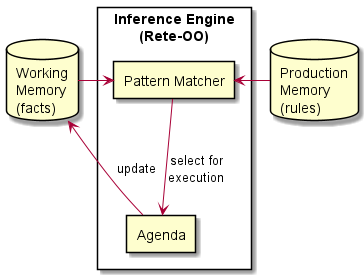
\includegraphics[width=0.55\textwidth]{Sections/images/components.png}}
    \caption{Drools components}
    \label{fig:Drools_components}
\end{figure}

To execute rules, Drools has four major components, as demonstrated in figure \ref{fig:Drools_components}.
The production memory contains the rules, and this will not change during an analysis session.
The rules are the focus of this thesis, and therefore, we will delve into much more detail later on these.


In Forgy's\cite{forgy1989rete} overview of a rete algorithm, the following steps occur.
\begin{enumerate}
    \setlength\itemsep{0em}
    \item Match: Evaluate the Left-hand sides (LHS) of the productions to determine which are satisfied given the current contents of working memory.
    \item Conflict resolution: Select one production with a satisfied LHS; halt the interpreter if no productions have satisfied LHSs.
    \item Act: Perform the actions in the RHS of the selected production.
    \item Re-evaluate: Go To 1.
\end{enumerate}

\begin{figure}
    \centering
    \fbox{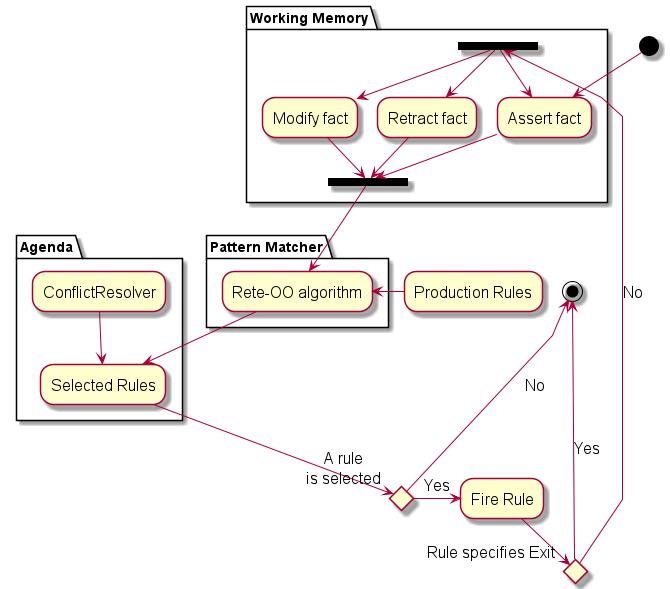
\includegraphics[width=0.70\textwidth]{Sections/images/InferenceLoop.png}}
    \caption{Drools inference loop}
    \label{fig:Drools_inference_loop}
\end{figure}

Figure \ref{fig:Drools_inference_loop} shows more detail of how these components interact within Drools to infer a conclusion.
First, Drools asserts facts in the working memory.
The working memory contains the current state of the facts, which triggers the inference engine.
Using the Rete-OO algorithm, the pattern matcher will examine both the working memory and a representation of the rules from the production memory to determine which rules are true.
Drools will then put the rules that match on the agenda.
It can be the case that many rules are concurrently true for the same fact assertion.
These rules conflict.
A conflict resolution strategy will decide which rule will fire in which order from the agenda.
The first rule on the agenda will fire.
If the rule modifies, retracts or asserts a fact, then the inference loop begins again.
We have inferred our conclusion if either a rule specifies to halt or no matching rules remain on the agenda.

The component we will be focussing on in this paper is the rules.
A rules file containing the rules is a text file, typically with a .drl extension.
The rules do not change during execution.
Drools stores the rules in the production memory.

This paper will ignore the rule file components \texttt{package}, \texttt{import}, \texttt{global}, \texttt{declare}, \texttt{function}, and \texttt{query}.

We will now examine the anatomy of a rule.
A rule consists of 3 parts: attributes, conditions, and consequences.
Attributes are optional hints to the inference engine as to how to examine a rule.
The conditional, ``\texttt{when}'', or left-hand side (LHS) of the rule statement is a block of conditions that must, in the aggregate, return true for the asserted fact. 
If true, then the rule is placed on the agenda.
The actions, consequences, ``\texttt{then}'', or right-hand side (RHS) of the rule statement contains actions to be executed when the rule is selected.

The LHS is a predicate statement made up of some patterns.
The patterns evaluate facts from the working memory.
The pattern can match against the existence of facts or facts with matching property conditions.
Connectives, such as \texttt{not}, \texttt{and}, and \texttt{or} can combine patterns.
The patterns apply to individual facts rather than the group, thus can be seen as first-order predicates.

Variables can be bound to facts that match these patterns for use later in the LHS or for updating the working memory on the RHS.

Drools offers more options for the LHS.
We have limited the scope of this paper to the features described thus far.

The RHS can contain arbitrary code that will execute when a rule is selected.
However, its primary purpose is to adjust the state of truth in the working memory.
One can insert, modify, and retract facts in the working memory.
Modifying and retracting facts must be done on fact variable references bound in the LHS.
One can explicitly terminate the inference loop with a halt command.

\begin{figure}
    \centering
    \fbox{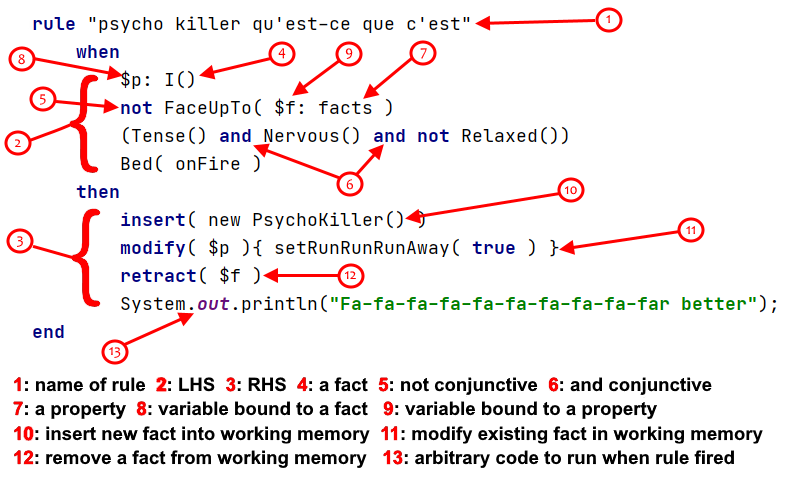
\includegraphics[width=0.95\textwidth]{Sections/images/DroolsRule2.png}}
    \caption{Drools rule breakdown}
    \label{fig:Drools_Rule_Breakdown}
\end{figure}

\subsubsection{An Explanatory Example}
Listing \ref{listing:drl_file} shows an example of a .drl file taken from the Drools sample code.

\noindent\begin{minipage}{\textwidth}
    \begin{lstlisting}[language={[drl]Drools}, caption=Example Drools file, captionpos=b, label=listing:drl_file]
    package org.drools.examples.honestpolitician

    import org.drools.examples.honestpolitician.Politician;
    import org.drools.examples.honest politician.Hope;
    
    rule "We have an honest Politician"
        salience 10
        when
            exists( Politician( honest == true ) )
        then
            insertLogical( new Hope() );
    end
    
    rule "Hope Lives"
        salience 10
        when
            exists( Hope() )
        then
            System.out.println( "Hurrah!!! Democracy Lives" );
    end
    
    rule "Hope is Dead"
        when
            not( Hope() )
        then
            System.out.println( "We are all Doomed!!! Democracy is Dead" );
    end
    
    rule "Corrupt the Honest"
        when
            $p : Politician( honest == true )   
            exists( Hope() )
        then
            System.out.println( "I'm an evil corporation and I have corrupted " + $p.getName() );
            modify( $p ) { 
                setHonest( false ) 
            }
    end
    \end{lstlisting}
\end{minipage}

Listing \ref{listing:drl_file} gives the Drools engine instructions on what actions to take when something changes the working memory.
This toy example reacts to when the working memory has an honest politician added. 
It prints a message celebrating the existence of said politician.
It then corrupts her and gloats in a message.
Finally, it prints a message of despair.
The code in Listing \ref{listing:drl_file} does the following: 
\begin{enumerate}[topsep=2pt,itemsep=2pt,partopsep=2pt, parsep=2pt]
    \setlength\itemsep{0em}
    \item On line 1, the \texttt{package} statement identifies the rule file.
    \item On lines 3 and 4, the \texttt{import} statements describe which facts are available for use.
    \item The ``We have an honest Politician'' rule on line 6 does the following:
    \begin{enumerate}[topsep=2pt,itemsep=2pt,partopsep=2pt, parsep=2pt]
        \setlength\itemsep{0em}
        \item On line 7, using the \texttt{salience} attribute, the rule is set to be run before other rules with a lower \texttt{salience}.
        \item On line 9, the rule checks working memory for \texttt{Politician} facts with the \texttt{honest} property equal to \texttt{true}.
        \item On line 11, if found, a \texttt{Hope} fact is inserted into the working memory.
    \end{enumerate}
    \item The ``Hope Lives'' rule on line 14 does the following:
    \begin{enumerate}[topsep=2pt,itemsep=2pt,partopsep=2pt, parsep=2pt]
        \setlength\itemsep{0em}
        \item Line 17 check if any \texttt{Hope} facts exist.
        \item On line 19, if found, it prints a message.
    \end{enumerate}
    \item The ``Hope is Dead'' rule on line 22 does the following:
    \begin{enumerate}[topsep=2pt,itemsep=2pt,partopsep=2pt, parsep=2pt]
        \setlength\itemsep{0em}
        \item On line 24, it checks that no \texttt{Hope} facts exist.
        \item On line 26, if it finds no facts, then it prints a message.  
    \end{enumerate}
    \item The ``Corrupt the Honest'' rule on line 29 does the following:
    \begin{enumerate}[topsep=2pt,itemsep=2pt,partopsep=2pt, parsep=2pt]
        \setlength\itemsep{0em}
        \item Line 31 checks for any \texttt{Politician} facts with the \texttt{honest} property equal to \texttt{true} and sets them to the variable \texttt{\$p}.
        \item Line 32 checks if any \texttt{Hope} facts exist.
        \item If both \texttt{Hope} and \texttt{Politician} facts are found, on line 34, it prints a message including the \texttt{\$p} variables name.
        \item On lines 35 to 37, it modifies the fact in working memory bound to the variable \texttt{\$p} to change its \texttt{honest} property.
    \end{enumerate}
\end{enumerate}